\documentclass[11pt,a4paper]{article}

\usepackage[margin=2.5cm]{geometry}
\usepackage{amsmath}
\usepackage{amssymb}
\usepackage{booktabs}
\usepackage{graphicx}
\usepackage[colorlinks=true,linkcolor=black,citecolor=blue,urlcolor=blue]{hyperref}

% thebibliography prints its own unnumbered "References" heading; the numbered
% \section{References} already provides it, so the next starred heading is
% swallowed once (star and title consumed together) and the sections after the
% bibliography keep the normal \section.
\makeatletter
\newcommand{\swallownextsectionstar}{%
  \let\originalsection\section
  \renewcommand{\section}{\@ifnextchar*{\swallowsectionstar}{\originalsection}}}
\def\swallowsectionstar*#1{\let\section\originalsection}
\makeatother

\title{\textbf{Optimised Dense Matrix Multiplication and Sparse CSR
Multiplication:\\ An Empirical Study of Optimisation and Structure
Effects}\thanks{Generative AI tools were utilized solely to refine the
stylistic quality, grammar, and technical phrasing of this report.}\\
\vspace{0.5cm}
\Large Big Data --- Bachelor's Degree in Data Science and Engineering (ULPGC)}

\author{\textbf{Aythami Lorenzo} \\[0.1cm]
\small University of Las Palmas de Gran Canaria \\
\small Code \& Data: \url{https://github.com/aythamilorenzo/bigdata-individual-assignments}}
\date{October 2026}

\begin{document}

\maketitle

\begin{abstract}
We study the behavior of several matrix multiplication algorithms used for
dense and sparse square matrices: a basic $i$-$j$-$k$ triple loop reused from
a previous study, an $i$-$k$-$j$ loop reordering, a cache-blocked variant, and
a sparse-sparse product in compressed sparse row (CSR) storage computed with
Gustavson's row-wise algorithm. We perform an analysis of the following
elements: kernel-only runtime with warm-ups and repeated measurements
(median and interquartile range), peak resident memory, output densification
and the separately measured dense-to-CSR conversion cost, across sizes up to
$n = 1500$ and densities from 1\% to 50\%. Our experiments provide a
reproducible benchmark of
optimised and sparse multiplication algorithms across a variety of matrix
sizes and sparsity levels to guide future research in performance analysis of
data-intensive workloads. Based on our experiments, we recommend the $i$-$k$-$j$
reordering as the default dense kernel for row-major storage, cache blocking
for the largest sizes, and CSR multiplication only while the input sparsity
outweighs indexing, conversion and output-densification costs.
\end{abstract}

\tableofcontents
\newpage

\section{Introduction and objective}
\label{sec:introduction}

Matrix multiplication is a canonical workload for studying how algorithms,
memory hierarchy and data structure interact. Assignment 1 established the
behavior of a basic $O(n^3)$ triple-loop multiplication as $n$ grows; this
study extends that baseline in the two directions required by the
assignment: \textbf{Part A (dense optimisation)} adds a loop reordering to
$i$-$k$-$j$ and a cache-blocked variant on top of the validated
$i$-$j$-$k$ baseline (three dense methods in total), and \textbf{Part B
(sparse matrices)} implements a sparse-sparse product in compressed sparse
row (CSR) storage, compared with a dense method on matched logical inputs at
several declared densities.

\paragraph{Research questions.}
\emph{RQ1:} how do the selected optimisations affect the runtime and memory of
dense multiplication as $n$ grows?
\emph{RQ2:} under which tested sparsity conditions does the sparse
representation outperform the dense method, and where do indexing, conversion
and output-densification costs erode it?

\section{Background}
\label{sec:background}

The basic dense algorithm multiplies two $n \times n$ matrices stored in
row-major order with three nested loops. The $i$-$j$-$k$ order accumulates
each output entry with a contiguous traversal of a row of $A$ but a strided
(column) traversal of $B$. Reordering the loops to $i$-$k$-$j$ keeps both
$B$ and the output contiguous~\cite{higham2002}; cache blocking (tiling)
restricts the loops to block-sized tiles so that working sets stay resident
in cache~\cite{lam1991}. Both variants retain $O(n^3)$ arithmetic work.

In compressed sparse row (CSR) storage each row lists the column indices and
values of its nonzero entries plus a row-pointer
array~\cite{saad2003}. One $n \times n$ matrix then costs
$12\,\mathrm{nnz} + 4(n+1)$ bytes with 8-byte float64 values and 4-byte
integer indices and pointers, versus $8n^2$ bytes dense ($24n^2$ bytes for
three dense matrices). Gustavson's row-wise algorithm multiplies sparse
inputs in time proportional to the nonzero counts rather than $n^3$: for
output row $i$ it performs
$\sum_{k \in \mathrm{supp}(A_i)} \mathrm{nnz}(B_k)$ scatter operations over
a dense accumulator row, plus one $O(n)$ sweep of that accumulator per output
row~\cite{gustavson1978}.

\section{Methodology}
\label{sec:methodology}

\subsection{Implementations}

All implementations are sequential, use double (float64) precision and are
written in Java 17. The $i$-$j$-$k$ baseline, the matrix domain and the
measurement harness are reused from assignment 1 and validated by its test
suite; this study adds three methods: the loop reordering
\texttt{triple\_loop\_ikj\_dense} (contiguous accesses to $B$ and the
output), the cache-blocked \texttt{blocked\_ijk\_dense} ($i$-$k$-$j$ in
$64 \times 64$ tiles, 32~KB per tile of $B$, block size fixed for the
campaign), and \texttt{sparse\_csr\_gustavson} --- Gustavson's algorithm on
canonical CSR (strictly increasing column indices per row) with a reusable
dense accumulator outside the timed region.

\subsection{Inputs and environment}

The dense methods of Part A multiply the shared inputs of assignment 1
(little-endian float64, row-major, seed 42, values uniform in $[0,1)$) plus
$n = 1500$. Part B generates declared-density inputs at
$\{1, 5, 10, 20, 50\}\%$ nonzero entries (positions uniformly without
replacement, values uniform in $[0,1)$, seeds per configuration in
\texttt{inputs\_manifest.csv}); for every $(n, \textit{density})$ the CSR
kernel and the dense comparison multiply the identical bytes. Experiments
ran inside WSL2 (Ubuntu 26.04) on an Intel Core i7-10750H (6 cores /
12 threads) with 16~GB DDR4, OpenJDK 17.0.20.1, Maven 3.9.12 and Python
3.14.4 (numpy 2.5.3, pandas 3.0.6, matplotlib 3.11.2).

\subsection{Measurement protocol}

The timer surrounds only the multiplication kernel: input loading,
dense-to-CSR conversion and the result checksum are outside the timed
region. Each configuration runs 3 warm-up repetitions (recorded, excluded)
then 7 measured repetitions on \texttt{System.nanoTime()}; every raw sample
is kept and medians with interquartile ranges are reported. Multiplications
shorter than 2~ms are batched and reported per multiplication. Budgets are
60~s per multiplication and about 2~GB of memory, overruns being reported as
results. Peak resident memory comes from \texttt{/proc/self/status}
(\texttt{VmHWM}), peak heap from \texttt{MemoryPoolMXBean}; theoretical
storage is reported alongside as a different quantity.

\subsection{Correctness}

Every optimised kernel is validated against the baseline on identity, zero,
known-answer $3 \times 3$ and seeded random matrices (JUnit);
independently, \texttt{correctness\_check.py} compares jar checksums
against a NumPy float64 reference ($\mathrm{rtol} = 10^{-9}$,
$\mathrm{atol} = 10^{-12}$), within which different summation orders
legitimately differ.

\section{Results}
\label{sec:results}

The campaign produced 230 raw dense samples (Part A) and 360 raw sparse
samples (Part B), each configuration with 3 warm-ups plus 7 measured
repetitions. All tables report the median of the 7 measured repetitions.

\subsection{Part A: dense optimisation}

Table~\ref{tab:dense-times} gives the kernel time per multiplication for
every size reached by each method. The baseline completed $n = 1000$ in
15.2~s and its single probe at $n = 1500$ exceeded the declared 60~s budget:
the overrun itself is the result. Both optimised methods completed
$n = 1500$ (1.7~s and 2.7~s). Figure~\ref{fig:dense-time} shows the growth
curves, and Figure~\ref{fig:dense-speedup} re-expresses the same
measurements as speedups over the baseline.

\begin{table}[t]
\centering
\caption{Median kernel time per multiplication (seconds) for the three dense
methods. ``budget'' marks the configuration whose probe exceeded 60~s.}
\label{tab:dense-times}
\begin{tabular}{rccc}
\toprule
$n$ & $i$-$j$-$k$ baseline & $i$-$k$-$j$ reordering & cache blocking \\
\midrule
100   & 0.0018  & 0.0005  & 0.0023 \\
200   & 0.0167  & 0.0035  & 0.0044 \\
500   & 0.358   & 0.0487  & 0.0710 \\
1000  & 15.17   & 0.613   & 0.536 \\
1500  & budget  & 2.69    & 1.72 \\
\bottomrule
\end{tabular}
\end{table}

\begin{figure}[t]
\centering
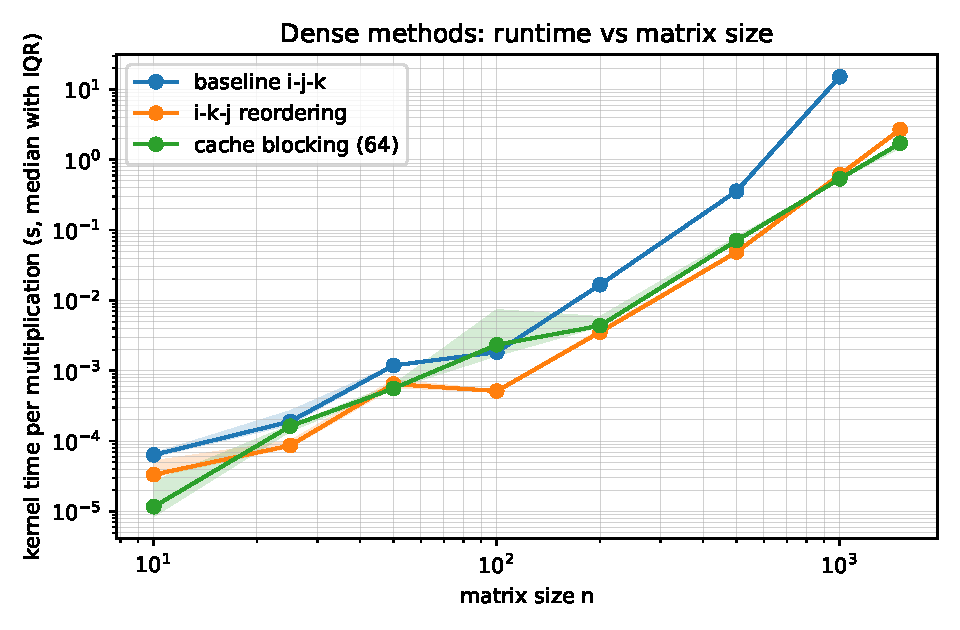
\includegraphics[width=0.72\linewidth]{figures/median_time_vs_size.pdf}
\caption{Kernel time per multiplication versus matrix size (median with IQR,
log--log), the three dense methods.}
\label{fig:dense-time}
\end{figure}

\begin{figure}[t]
\centering
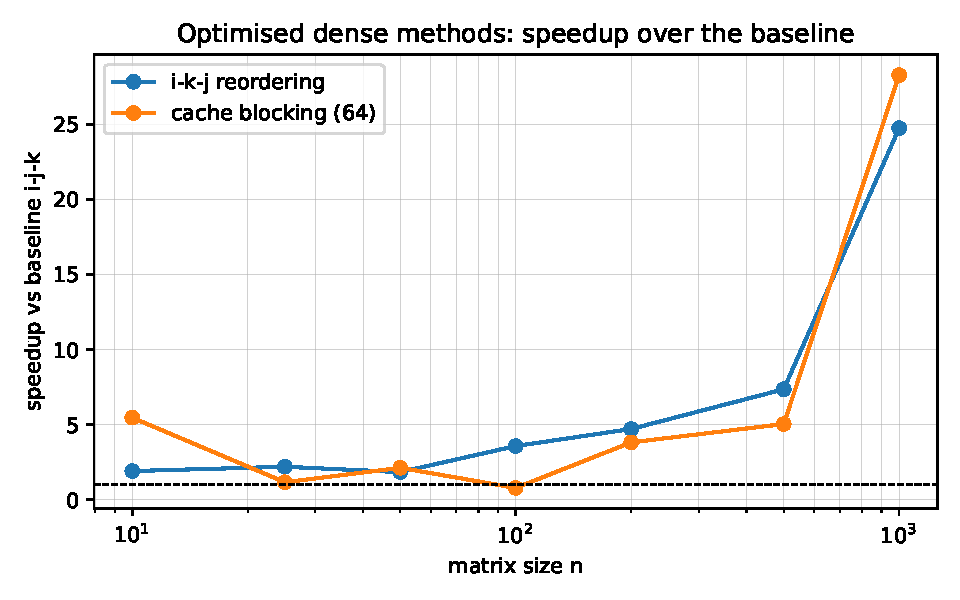
\includegraphics[width=0.72\linewidth]{figures/speedup_vs_baseline.pdf}
\caption{Speedup of the two optimised dense methods over the baseline
$i$-$j$-$k$ kernel versus matrix size.}
\label{fig:dense-speedup}
\end{figure}

\subsection{Part B: sparse multiplication}

Table~\ref{tab:sparse-speedup} shows the matched comparison: the ratio of
the dense $i$-$k$-$j$ time over the CSR kernel time on identical logical
matrices (values above 1.0 mean the sparse representation wins). The CSR
kernel wins by two orders of magnitude at $n = 1000$ and 1\% density
(101.8$\times$), and its advantage contracts monotonically as density grows,
reaching $1.8\times$ at 50\% density for $n = 1000$. At the smallest size
($n = 100$) fixed per-call overheads dominate: the dense method is faster
from 10\% density onwards. Figure~\ref{fig:sparse-time} shows the absolute
kernel times behind these ratios, and Figure~\ref{fig:sparse-speedup} the
ratios themselves.

\begin{table}[t]
\centering
\caption{Matched comparison: dense $i$-$k$-$j$ time divided by CSR kernel
time (median); values above 1.0 favour the sparse representation. The
largest size is compared at the declared probe density 10\% only.}
\label{tab:sparse-speedup}
\begin{tabular}{rccccc}
\toprule
$n$ \textbackslash\ density \% & 1 & 5 & 10 & 20 & 50 \\
\midrule
100  & 4.0   & 1.3  & 0.7  & 0.8  & 0.4 \\
500  & 34.3  & 7.8  & 8.6  & 4.5  & 1.2 \\
1000 & 101.8 & 35.3 & 18.7 & 7.8  & 1.8 \\
2000 & ---   & ---  & 41.2 & ---  & --- \\
\bottomrule
\end{tabular}
\end{table}

\begin{figure}[t]
\centering
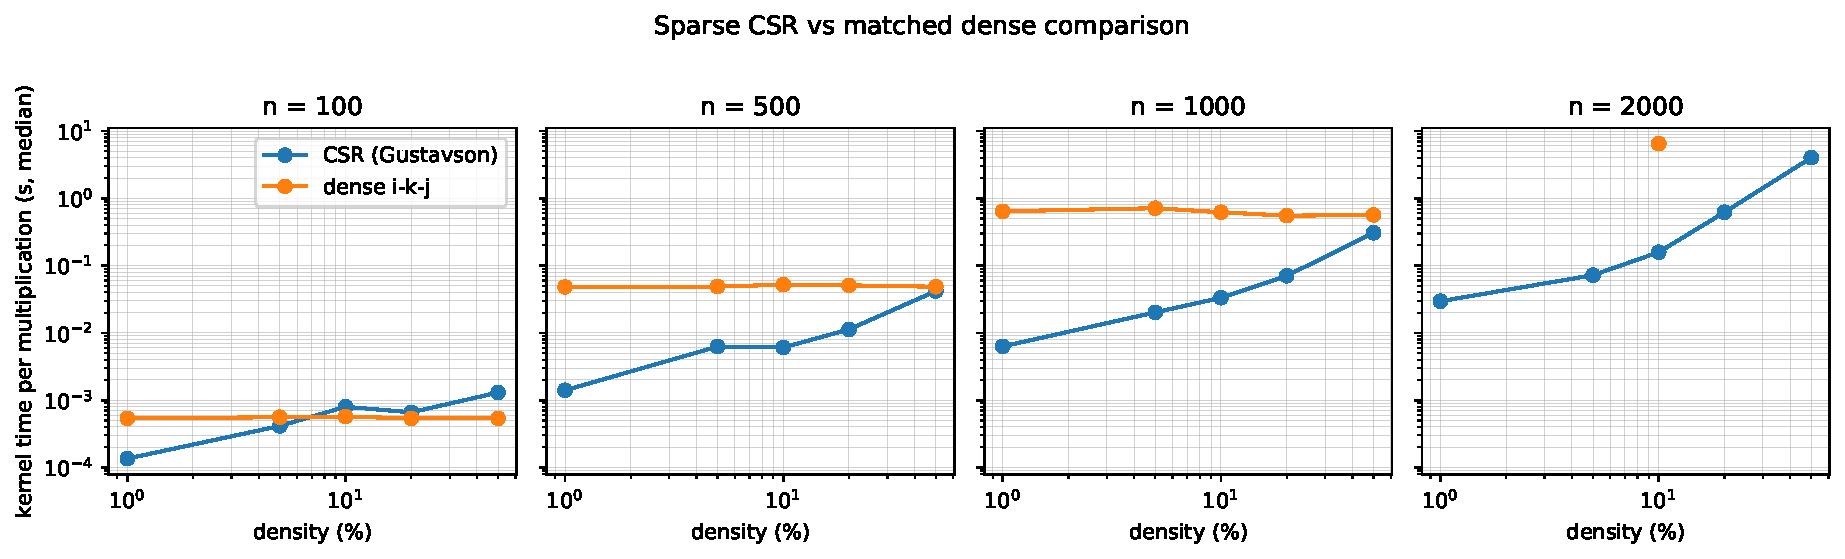
\includegraphics[width=\linewidth]{figures/sparse_time_vs_density.pdf}
\caption{CSR kernel versus the matched dense comparison: kernel time
versus declared density, per size (log--log).}
\label{fig:sparse-time}
\end{figure}

\begin{figure}[t]
\centering
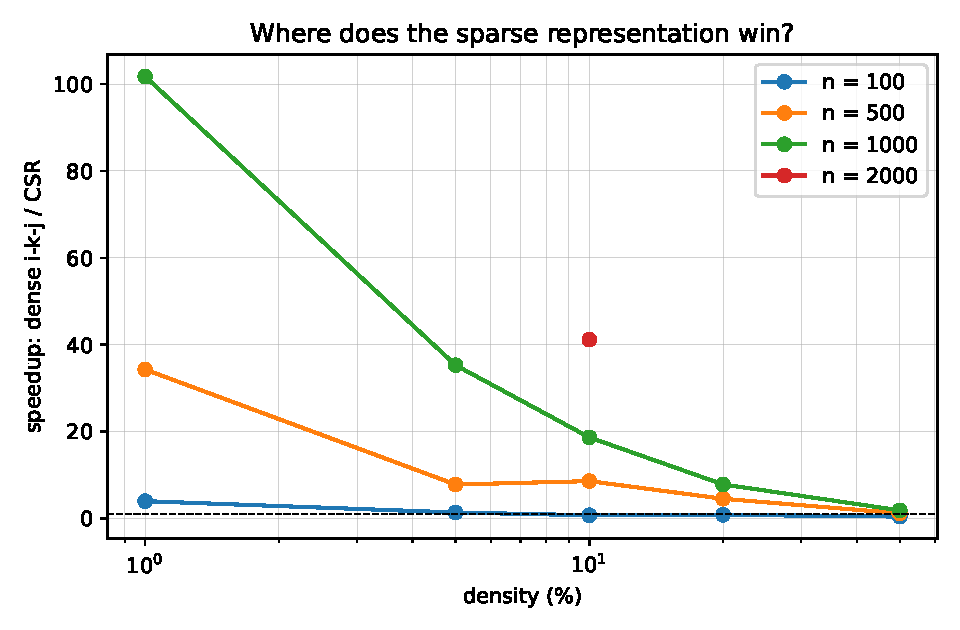
\includegraphics[width=0.72\linewidth]{figures/sparse_speedup_vs_density.pdf}
\caption{Dense $i$-$k$-$j$ time divided by CSR kernel time versus declared
density, per size; above the dashed line the sparse representation wins.}
\label{fig:sparse-speedup}
\end{figure}

Table~\ref{tab:nnz} reports the realised output densification: the product
of two matrices at density $d$ has expected nonzero fraction
$1 - (1 - d^2)^n$, which approaches 1 rapidly. At $n = 1000$ a 5\% input
already yields a 92\% dense output, so the sparse structure of the inputs
does not propagate to the product. Figure~\ref{fig:nnz-growth} plots the
realised output fraction against the declared input density.

\begin{table}[t]
\centering
\caption{Median percentage of nonzero entries in the product $C$ (output
density), from the \texttt{nnz\_c} column of the raw CSV.}
\label{tab:nnz}
\begin{tabular}{rccccc}
\toprule
$n$ \textbackslash\ density \% & 1 & 5 & 10 & 20 & 50 \\
\midrule
100  & 1.1  & 21.3 & 62.1 & 98.8 & 100 \\
500  & 4.9  & 71.6 & 99.3 & 100  & 100 \\
1000 & 9.6  & 91.8 & 100  & 100  & 100 \\
2000 & 18.1 & 99.3 & 100  & 100  & 100 \\
\bottomrule
\end{tabular}
\end{table}

\begin{figure}[t]
\centering
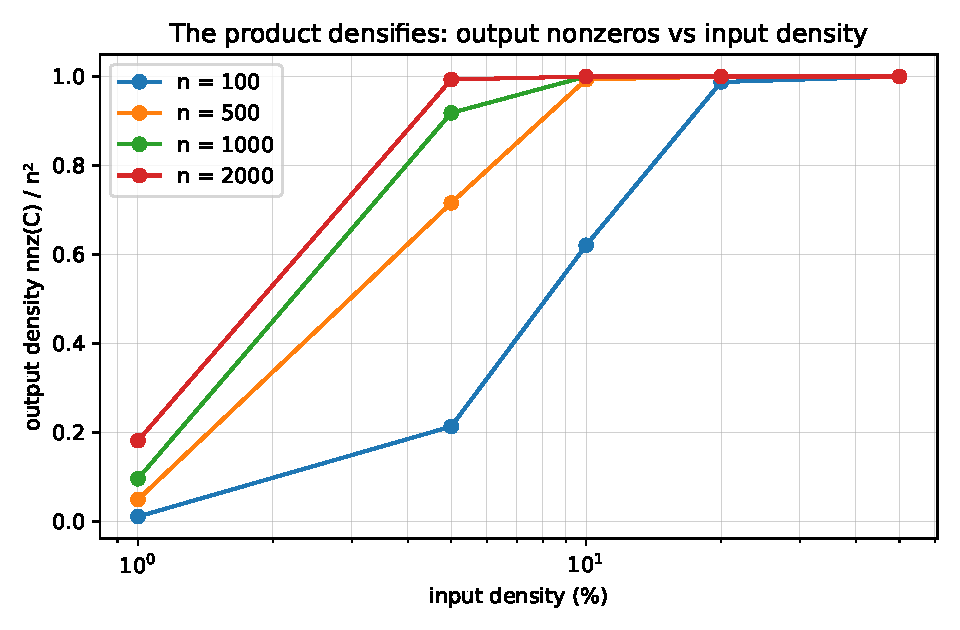
\includegraphics[width=0.72\linewidth]{figures/nnz_growth_vs_density.pdf}
\caption{Output densification: fraction of nonzeros in $C$ versus input
density, per size.}
\label{fig:nnz-growth}
\end{figure}

The separately measured dense-to-CSR conversion (Table~\ref{tab:conversion})
costs 53--107~ms at $n = 1000$ and 80--179~ms at $n = 2000$ --- one to two
orders of magnitude \emph{more} than the CSR kernel itself at low density
(6.3~ms at $n = 1000$, 1\%). A pipeline starting from dense files pays this
once per pair of matrices; natively sparse inputs never pay it.
Figure~\ref{fig:conversion} compares the two components directly.

\begin{table}[t]
\centering
\caption{Median dense-to-CSR conversion time (milliseconds), measured
outside the kernel timing.}
\label{tab:conversion}
\begin{tabular}{rccccc}
\toprule
$n$ \textbackslash\ density \% & 1 & 5 & 10 & 20 & 50 \\
\midrule
100  & 4.8  & 4.0  & 5.3  & 4.4  & 5.4 \\
500  & 21.3 & 25.0 & 26.8 & 26.3 & 30.3 \\
1000 & 53.4 & 56.2 & 60.9 & 106.6 & 84.6 \\
2000 & 80.1 & 102.6 & 123.2 & 126.5 & 179.4 \\
\bottomrule
\end{tabular}
\end{table}

\begin{figure}[t]
\centering
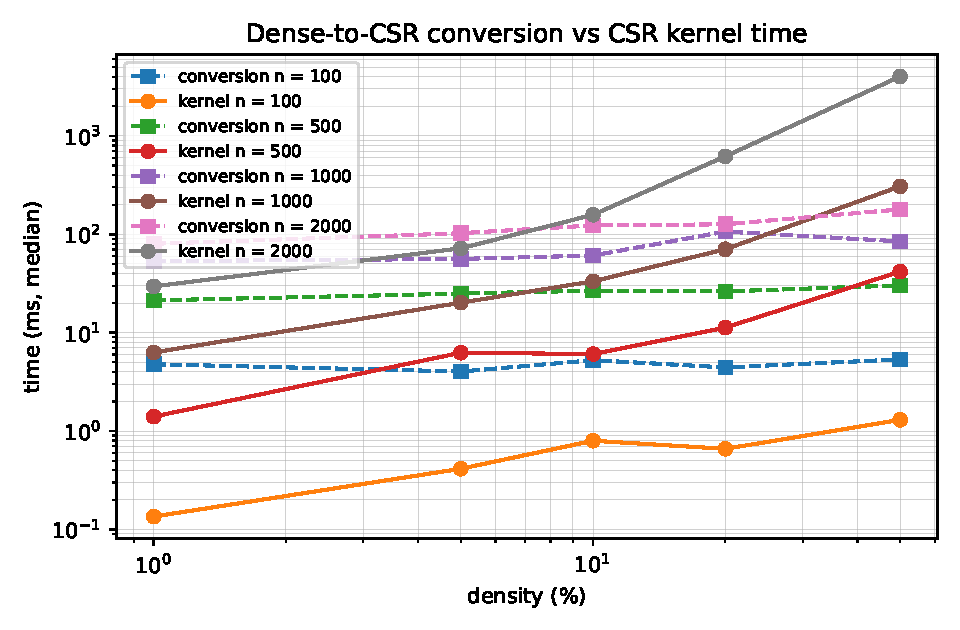
\includegraphics[width=0.72\linewidth]{figures/conversion_vs_kernel.pdf}
\caption{Dense-to-CSR conversion time versus CSR kernel time (medians,
log--log), per size and density.}
\label{fig:conversion}
\end{figure}

Charging that conversion once, the end-to-end ratio of the sparse pipeline
(conversion + kernel) over the dense multiplication is shown in
Figure~\ref{fig:pipeline}. It stays above~1 at every tested density for
$n \ge 1000$ ($1.4$--$10.7\times$, and $23.1\times$ at the $n = 2000$
probe) and at $n = 500$ up to 20\% ($1.4$--$2.1\times$); it falls below~1
only at $n = 100$ ($0.08$--$0.13\times$) and at the densest configuration
of $n = 500$ ($0.67\times$).

\begin{figure}[t]
\centering
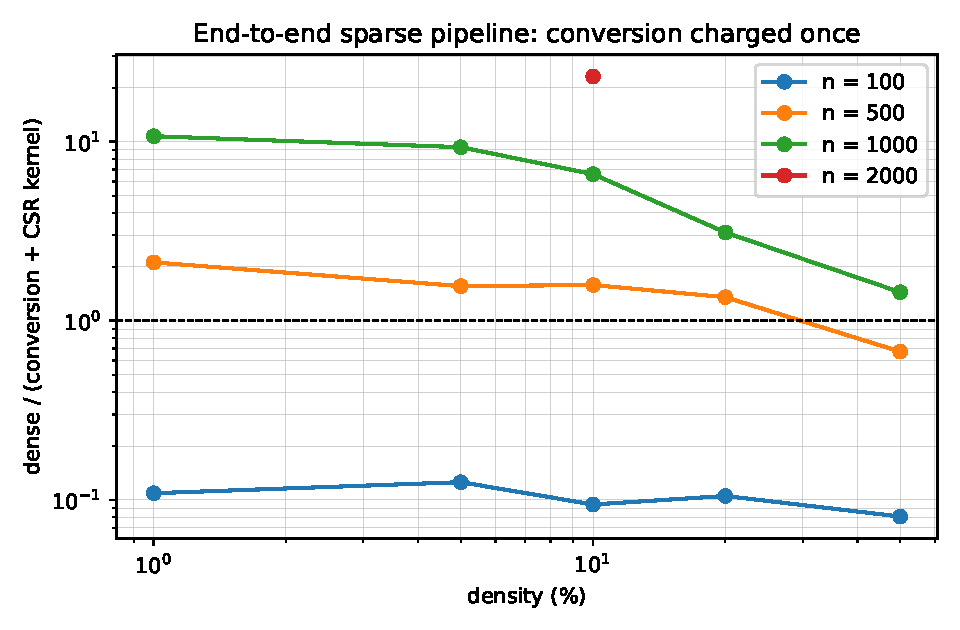
\includegraphics[width=0.72\linewidth]{figures/pipeline_end_to_end.pdf}
\caption{End-to-end sparse pipeline versus dense: dense time divided by
(conversion + CSR kernel), so the one-off conversion is charged once; above
the dashed line the pipeline wins.}
\label{fig:pipeline}
\end{figure}

\subsection{Memory}

Peak resident memory (Figure~\ref{fig:memory}) is dominated by the JVM floor
(about 44~MiB at small sizes): Part A measured 112~MiB at $n = 1000$ and
about 142~MiB at $n = 1500$, essentially identical for the three methods ---
the optimisations change the time, not the space. In Part B, peak RSS grows
with the realised nonzero counts (228--455~MiB at $n = 2000$), because the
run also materialises the dense input files it loads before conversion.

\begin{figure}[t]
\centering
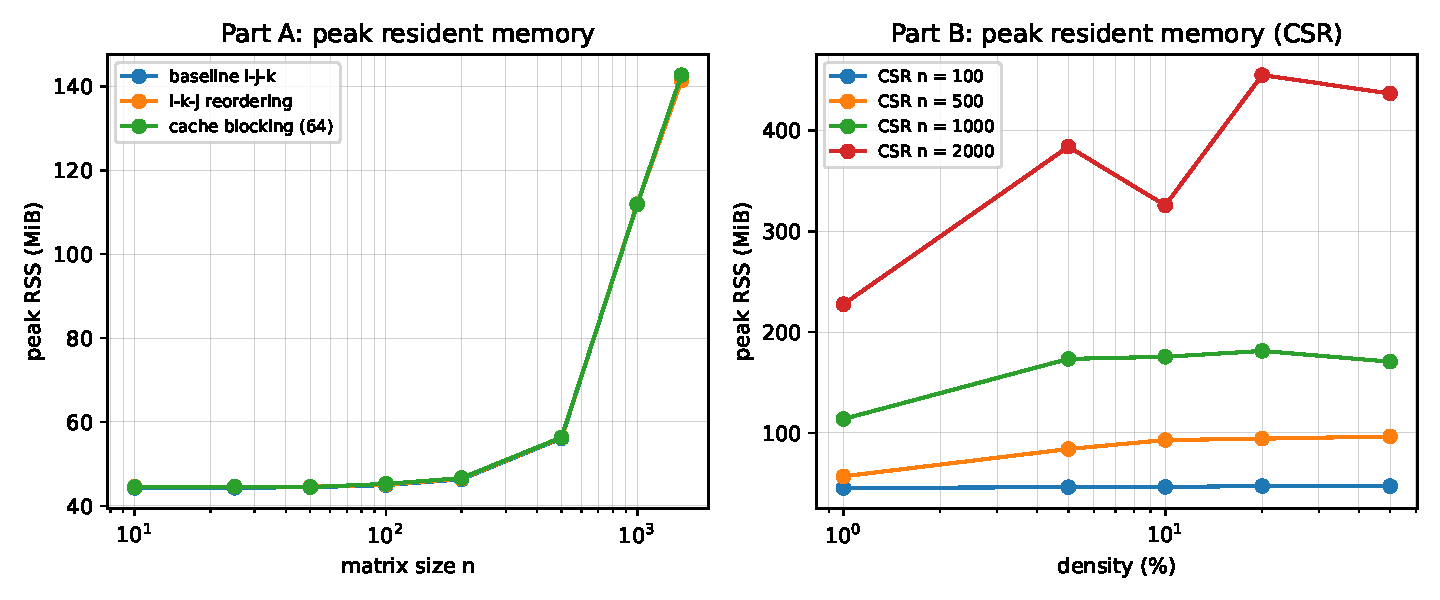
\includegraphics[width=\linewidth]{figures/peak_rss_all.pdf}
\caption{Peak resident memory versus size (Part A, left) and versus density
for the CSR runs (Part B, right), medians per configuration.}
\label{fig:memory}
\end{figure}

Figure~\ref{fig:storage} places that measured peak next to the theoretical
structural storage --- $24n^2$ bytes for three dense matrices and
$12\,\mathrm{nnz} + 4(n+1)$ bytes per CSR matrix. The roughly constant gap
at small sizes is the JVM floor, and in Part B the peak additionally
includes the dense input files materialised before conversion: the two
curves are different quantities, reported side by side and never as one
measurement.

\begin{figure}[t]
\centering
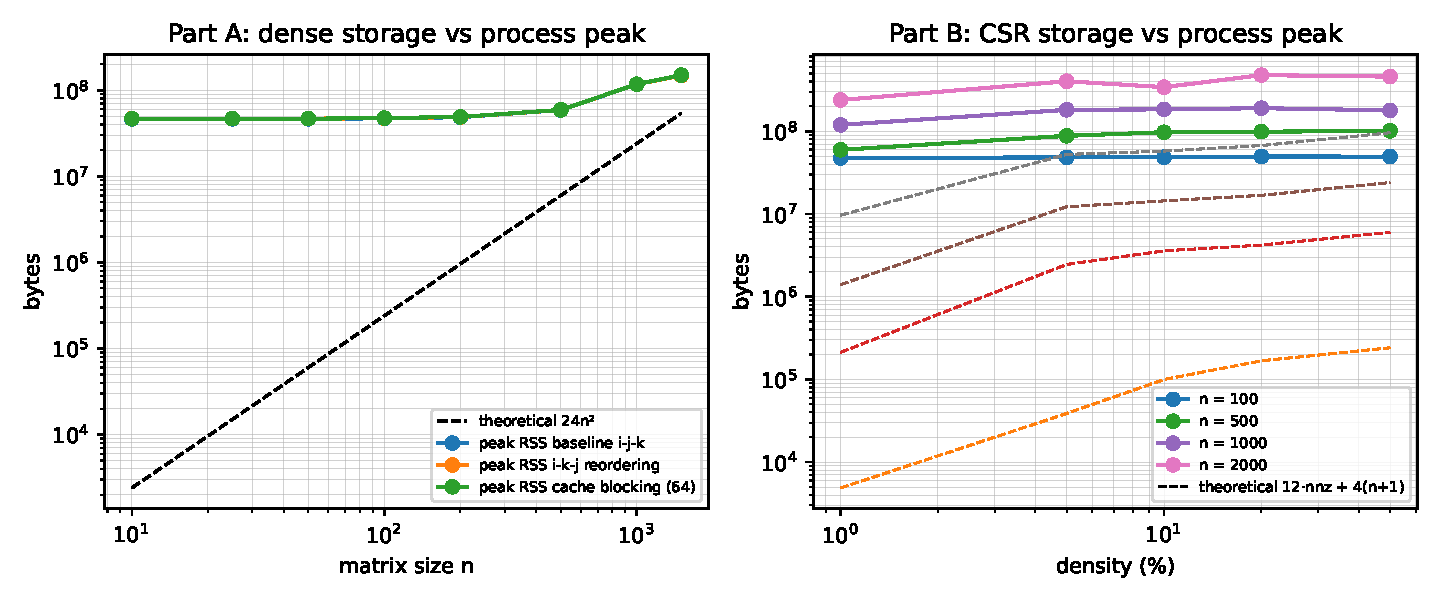
\includegraphics[width=\linewidth]{figures/storage_theoretical_vs_observed.pdf}
\caption{Theoretical structural storage (dashed) versus measured peak
resident memory (solid) in bytes, log--log: Part A, dense $24n^2$ (left);
Part B, CSR storage per density (right).}
\label{fig:storage}
\end{figure}

\section{Discussion}
\label{sec:discussion}

\subsection{Effect of the optimisations (RQ1)}

The two dense optimisations act on the memory-access pattern, not on the
arithmetic: all three methods perform exactly $2n^3$ multiply--adds. The
baseline's strided column access to $B$ is the dominant cost; removing it
yields $4.7\times$ at $n = 200$, $7.4\times$ at $n = 500$ and $24.7\times$
at $n = 1000$ for the $i$-$k$-$j$ reordering alone
(Table~\ref{tab:dense-times}, Figure~\ref{fig:dense-speedup}). Cache
blocking is a second, smaller effect on top of the reordering: it ties plain
$i$-$k$-$j$ up to $n = 500$ (slightly slower at $n = 100$ and $n = 500$,
where tile bookkeeping is not yet repaid), then pulls ahead at the largest
sizes ($28.3\times$ versus $24.7\times$ at $n = 1000$; 1.72~s versus
2.69~s at $n = 1500$).

The cache hierarchy explains why blocking pays only at the largest sizes:
at $n = 1000$ the three dense matrices occupy 24~MB, more than the 12~MB
last-level cache of the i7-10750H, so the baseline's strided reads of $B$
become cache misses~\cite{frigo1999,hennessy2017}; the $i$-$k$-$j$ order
streams $B$ and the output through cache, and each $64 \times 64$ tile of
$B$ (32~KB) fits comfortably in the core's private 256~KB L2 cache for the
whole tile~\cite{lam1991} --- but the tile bookkeeping only repays itself
once the miss cost is large, i.e.\ at large $n$.

Below $n \approx 100$ differences are JIT and measurement noise
($0.8\times$--$5.5\times$), so no claim is made for small matrices. The
budget shows the impact: the baseline's probe at $n = 1500$ exceeded 60~s
while both optimised kernels finished in under 3~s, extending the largest
feasible size from $n = 1000$ to $n = 1500$ with identical peak RSS --- a
purely time effect.

\subsection{Effect of sparse storage and input structure (RQ2)}

Three separate effects pull in opposite directions:
\begin{enumerate}
    \item \textbf{Work scaling:} the CSR kernel's work grows with the
    nonzero counts, while the dense method always does $2n^3$ multiply--adds
    regardless of the values it reads --- dense comparison times are flat
    across densities at a given size (0.55--0.71~s at $n = 1000$). The sparse
    advantage is therefore maximal at low density: $101.8\times$ at
    $n = 1000$, 1\%.
    \item \textbf{Output densification:} the product is not sparse even when
    the inputs are --- its expected nonzero fraction $1 - (1 - d^2)^n$ reaches
    92\% at $n = 1000$, $d = 5\%$ and 100\% for $d \ge 10\%$ at that size
    (Table~\ref{tab:nnz}, Figure~\ref{fig:nnz-growth}). The kernel builds a
    nearly dense output while still paying per-nonzero indexing, and the CSR
    memory saving shrinks toward the dense figure. \emph{Input density alone
    never determines the outcome; the output structure matters just as
    much.}
    \item \textbf{Fixed per-call overheads:} the accumulator sweep and the
    output compaction cost $O(n^2)$ per multiplication even for a one-percent
    input, so at $n = 100$ the dense method wins from 10\% onwards
    ($0.7\times$, $0.8\times$, $0.4\times$).
\end{enumerate}
The crossover moves with size: at $n = 500$ the sparse kernel wins at every
tested density but only marginally at 50\% ($1.2\times$); at $n = 1000$ it
wins everywhere ($1.8\times$ at 50\%); at $n = 2000$ it wins by
$41.2\times$ at the 10\% probe density; at $n = 100$ the dense method wins
at 10\% and above.

Conversion deserves separate treatment, as the protocol requires: it costs
53--107~ms at $n = 1000$ against a 6.3~ms CSR kernel at 1\%, so for a
\emph{single} multiplication of dense-held inputs the conversion, not the
kernel, dominates that pipeline. It is paid once per pair of matrices and
can be amortised over repeated multiplications (kernel timing excludes it,
as declared); and even charged once at $n = 1000$, conversion + kernel
(59~ms at 1\%) stays an order of magnitude below the 640~ms dense
multiplication it replaces. Figure~\ref{fig:pipeline} charges it once at
every configuration: the advantage survives intact for all of $n \ge 1000$
and for $n = 500$ up to 20\%, and disappears exactly where the kernel itself
was already marginal --- $0.67\times$ at $n = 500$, 50\% and
$0.08$--$0.13\times$ at $n = 100$.

\subsection{Threats to validity}

Results are scoped to one machine, one JVM, sequential float64 Java kernels,
the tested sizes ($n \le 2000$), the tested densities (1--50\%) and the
declared block size of 64 (not tuned). Dense comparison rows at $n = 2000$
exist only at the declared 10\% probe density, justified by the observed
density-independence of dense runtime. Peak RSS includes the JVM floor and
the dense inputs materialised before conversion, so it is not a pure CSR
measurement; the theoretical storage columns give that quantity separately.

\section{Conclusions}
\label{sec:conclusions}

\paragraph{RQ1 --- dense optimisation.} Loop reordering to $i$-$k$-$j$ is
the highest-value change for row-major storage: it removes the strided access
to $B$ and delivers $24.7\times$ over the baseline at $n = 1000$ with no
tuning. Cache blocking pays off only at the largest tested sizes, where it
becomes the best method ($28.3\times$ at $n = 1000$; 1.72~s at $n = 1500$
where the baseline exceeds the 60~s budget). We recommend $i$-$k$-$j$ as the
default dense kernel and the blocked variant for the largest sizes, keeping
$i$-$j$-$k$ only as a reference; none of this changes memory usage.

\paragraph{RQ2 --- sparse multiplication.} The sparse CSR kernel helps when
\emph{all} of the following hold: the matrices are large ($n \ge 500$), the
input density is low to moderate ($\le 20\%$ gives $4.5$--$101.8\times$ in
our runs), and the inputs are available in (or cheaply convertible to) sparse
form. The advantage erodes through three measured mechanisms: growing output
densification, the $O(n^2)$ per-call floor that dominates small sizes, and
the conversion cost a dense-held pipeline pays once. At 50\% density it is
marginal ($1.2$--$1.8\times$) and at $n = 100$ the dense method wins from
10\% onwards: no percentage of zeros alone determines performance --- size,
output structure and input format decide together.

\paragraph{What remains open.} The block size was fixed, not swept; only CSR
and Gustavson's algorithm were tested (other formats such as ELL and COO
remain unexplored); the kernels are sequential, with parallelism left to the
next assignment; and the density grid stops at 50\%, so the crossover above
that point is not localised.

\section{References}
\swallownextsectionstar
\begin{thebibliography}{9}
    \bibitem{higham2002}
    N.~J. Higham, \emph{Accuracy and Stability of Numerical Algorithms},
    2nd~ed. SIAM, 2002.

    \bibitem{lam1991}
    M.~Lam, E.~E. Rothberg, and M.~D. Smith, ``The cache performance and
    optimizations of blocked algorithms,'' in \emph{Proc. 4th Int. Conf. on
    Architectural Support for Programming Languages and Operating Systems
    (ASPLOS)}, 1991, pp. 63--74.

    \bibitem{saad2003}
    Y.~Saad, \emph{Iterative Methods for Sparse Linear Systems}, 2nd~ed.
    SIAM, 2003.

    \bibitem{gustavson1978}
    F.~G. Gustavson, ``Two fast algorithms for dense matrices,''
    \emph{ACM Trans. Math. Software}, vol.~4, no.~3, pp. 250--259, 1978.

    \bibitem{frigo1999}
    M.~Frigo, C.~E. Leiserson, H.~H. Prokop, and S.~Ramachandran,
    ``Cache-oblivious algorithms,'' in \emph{Proc. 40th Annual Symposium on
    Foundations of Computer Science (FOCS)}, 1999, pp. 285--297.

    \bibitem{hennessy2017}
    J.~L. Hennessy and D.~A. Patterson, \emph{Computer Architecture: A
    Quantitative Approach}, 6th~ed. Morgan Kaufmann, 2017.
\end{thebibliography}

\section{Reproducibility materials}

All materials ship with this report: the Java (Maven) and Python sources;
the JUnit tests and the independent NumPy cross-check; the dense and sparse
input generators; the raw campaign CSVs (\texttt{dense\_time\_raw.csv},
\texttt{sparse\_time\_raw.csv}, \texttt{memory\_raw.csv} and
\texttt{run\_log.txt}); and the figure script plus figure PDFs. They are
attached as \texttt{Assignment02\_Lorenzo\_Materials.zip} to the
\texttt{assignment-02} release of the course repository. From the project
root, inside WSL2:

\begin{verbatim}
.venv/bin/python python/generate_inputs.py --sizes 1500
.venv/bin/python python/generate_sparse_inputs.py
mvn -q verify
mvn -q -DskipTests package
.venv/bin/python python/correctness_check.py
.venv/bin/python -m compileall python
.venv/bin/python python/run_experiments.py  # campaign
.venv/bin/python python/plot_results.py     # figures/*.pdf
\end{verbatim}

Exact toolchain versions and the full protocol are documented in
\texttt{README.md}. Runner exit codes: 0 (ok), 2 (invalid arguments), 3
(time budget exceeded), 4 (missing input files). The input binaries are
regenerated deterministically from seed 42 and are not shipped.
\url{https://github.com/aythamilorenzo/bigdata-individual-assignments}.

\end{document}
